% Options for packages loaded elsewhere
\PassOptionsToPackage{unicode}{hyperref}
\PassOptionsToPackage{hyphens}{url}
%
\documentclass[
  11pt,
]{article}
\usepackage{amsmath,amssymb}
\usepackage{lmodern}
\usepackage{iftex}
\ifPDFTeX
  \usepackage[T1]{fontenc}
  \usepackage[utf8]{inputenc}
  \usepackage{textcomp} % provide euro and other symbols
\else % if luatex or xetex
  \usepackage{unicode-math}
  \defaultfontfeatures{Scale=MatchLowercase}
  \defaultfontfeatures[\rmfamily]{Ligatures=TeX,Scale=1}
\fi
% Use upquote if available, for straight quotes in verbatim environments
\IfFileExists{upquote.sty}{\usepackage{upquote}}{}
\IfFileExists{microtype.sty}{% use microtype if available
  \usepackage[]{microtype}
  \UseMicrotypeSet[protrusion]{basicmath} % disable protrusion for tt fonts
}{}
\makeatletter
\@ifundefined{KOMAClassName}{% if non-KOMA class
  \IfFileExists{parskip.sty}{%
    \usepackage{parskip}
  }{% else
    \setlength{\parindent}{0pt}
    \setlength{\parskip}{6pt plus 2pt minus 1pt}}
}{% if KOMA class
  \KOMAoptions{parskip=half}}
\makeatother
\usepackage{xcolor}
\usepackage[margin=1in]{geometry}
\usepackage{graphicx}
\makeatletter
\def\maxwidth{\ifdim\Gin@nat@width>\linewidth\linewidth\else\Gin@nat@width\fi}
\def\maxheight{\ifdim\Gin@nat@height>\textheight\textheight\else\Gin@nat@height\fi}
\makeatother
% Scale images if necessary, so that they will not overflow the page
% margins by default, and it is still possible to overwrite the defaults
% using explicit options in \includegraphics[width, height, ...]{}
\setkeys{Gin}{width=\maxwidth,height=\maxheight,keepaspectratio}
% Set default figure placement to htbp
\makeatletter
\def\fps@figure{htbp}
\makeatother
\setlength{\emergencystretch}{3em} % prevent overfull lines
\providecommand{\tightlist}{%
  \setlength{\itemsep}{0pt}\setlength{\parskip}{0pt}}
\setcounter{secnumdepth}{-\maxdimen} % remove section numbering
\usepackage{indentfirst}
\usepackage{graphicx}
\usepackage{geometry}
\usepackage{subfigure}
\usepackage{amsmath}
\usepackage{listings}
\usepackage{tikz}
\usetikzlibrary{matrix}
\ifLuaTeX
  \usepackage{selnolig}  % disable illegal ligatures
\fi
\IfFileExists{bookmark.sty}{\usepackage{bookmark}}{\usepackage{hyperref}}
\IfFileExists{xurl.sty}{\usepackage{xurl}}{} % add URL line breaks if available
\urlstyle{same} % disable monospaced font for URLs
\hypersetup{
  pdftitle={Econometria I},
  pdfauthor={Lista de Exercícios 1 (Gabarito)},
  hidelinks,
  pdfcreator={LaTeX via pandoc}}

\title{Econometria I}
\author{Lista de Exercícios 1 (Gabarito)}
\date{PIMES/UFPE}

\begin{document}
\maketitle

\vspace{0.25in}

\hypertarget{problemas-conceituais}{%
\section{Problemas conceituais}\label{problemas-conceituais}}

\begin{enumerate}
\def\labelenumi{\arabic{enumi}.}
\item
  A resposta a estas questões podem ser encontradas no Greene, cap. 2
  (8a edição)

  \begin{enumerate}
  \def\labelenumii{\alph{enumii}.}
  \item
    Greene, pag. 20
  \item
    Greene, pag. 17
  \item
    Greene, pag. 22
  \item
    Greene, pag. 23
  \item
    Greene, pag. 25
  \end{enumerate}
\item
  A resposta a esta questão pode ser encontrada no Greene, cap.3 (8a
  edição), pag. 29.
\item
  Abaixo defninimos o modelo de regresão simples como
  \[y_i=\alpha + \beta x_i + \varepsilon_i\]

  \begin{enumerate}
  \def\labelenumii{\alph{enumii}.}
  \item
    Mostre que este modelo pode ser escrito equivalentemente em forma
    matricial como
    \(\mathbf{y}=\mathbf{X}\mathbf{\beta}+\mathbf{\varepsilon}\).
  \item
    Escreva a expressão para \(\mathbf{b}\), o estimador de MQO, em
    termos matriciais. Verifique que esta forma é equivalente às
    expressões \[\hat{\alpha}=\bar{y}-\hat{\beta}\] e
  \end{enumerate}

  \[\hat{\beta}=\frac{\frac{1}{n}\sum_{i=1}^n{x_iy_i}-\left(\frac{1}{n}\sum_{i=1}^n{x_i}\right)\left(\frac{1}{n}\sum_{i=1}^n{y_i}\right)}{\frac{1}{n}\sum_{i=1}^n{x_i^2}-\left(\frac{1}{n}\sum_{i=1}^n{x_i}\right)^2}\]
\item
  A resposta a esta questão pode ser encontrada no Greene, cap.3 (8a
  edição), pag. 36.
\item
  Na regressão \(\mathbf{y}\) em \(\mathbf{i}\) e \(\mathbf{X}\), os
  coeficientes de \(\mathbf{X}\) são
  \(\mathbf{b} = (\mathbf{X'M^0X})^{-1}\mathbf{X'M^0y}\).
  \(\mathbf{M}^0 = \mathbf{I} - \mathbf{i}(\mathbf{i'i})^{-1}\mathbf{i}'\)
  é a matriz que transforma as observações em desvios em relação à média
  das colunas. Como \(\mathbf{M}^0\) é idempotente e simétrica, podemos
  escrever a equação anterior como
  \([(\mathbf{X'M^0}')(\mathbf{M^0X})]^{-1}(\mathbf{X'M^0}')(\mathbf{M^0y})\),
  o que implica que a regressão de \(\mathbf{M^0y}\) em \(M^0X\) produz
  os coeficientes de inclinação por mínimos quadrados. Caso somente
  \(\mathbf{X}\) seja transformado em desvios, teríamos
  \([(\mathbf{X'M^0}')(\mathbf{M^0X})]^{-1}(\mathbf{X'M^0}')\mathbf{y}\)
  mas, obviamente, é idêntico ao caso anterior. Entretanto, caso somente
  \(\mathbf{y}\) seja transformado, o resultado é
  \((\mathbf{X'X})^{-1}\mathbf{X'M^0y}\), o qual é muito provavelmente
  diferente.
\item
  Considere o modelo \(\mathbf{y}=\mathbf{X}\mathbf{b}+\mathbf{e}\) A
  partir das definições \(SST=\sum_{i=1}^n{(y_i-\bar{y})^2}\),
  \(SSR=\sum_{i=1}^n{(\hat{y}_i-\bar{y})^2}\) e
  \(SSE=\mathbf{e}'\mathbf{e}=\sum_{i=1}^n{e_i^2}\), responda as
  seguintes questões:

  \begin{enumerate}
  \def\labelenumii{\alph{enumii}.}
  \item
    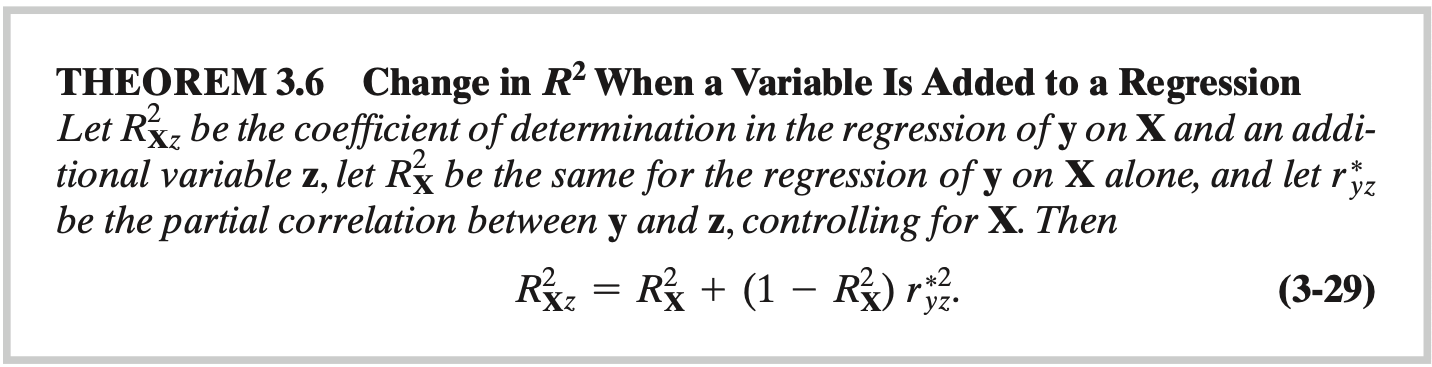
\includegraphics{/Users/henriquefonseca/Desktop/temp/Rmarkdown-practice/henriqueveras.github.io/files/Econometrics/Lecture Notes/2/theorem_3.6.png}
  \item
    A resposta a esta questão pode ser encontrada no Greene, cap.3 (8a
    edição), pag. 45.
  \end{enumerate}
\end{enumerate}

\hypertarget{problemas-pruxe1ticos}{%
\section{Problemas práticos}\label{problemas-pruxe1ticos}}

Considere a seguinte base de dados:

\[\mathbf{X}=
\begin{bmatrix} 
  1 &   4 &  2 \\
  1 &   7 &  6 \\
  1 &   2 &  9  \\
  1 &   1 &  4  \\
  \end{bmatrix}, 
% 
\mathbf{y}=
\begin{bmatrix} 
    6  \\
    11 \\
    4  \\
    3 \\
\end{bmatrix}\]

\begin{enumerate}
\def\labelenumi{\arabic{enumi}.}
\item
  Com base nos dados fornecidos, as quantidades solicitadas são

  \begin{enumerate}
  \def\labelenumii{\alph{enumii}.}
  \item
    \(\mathbf{X}'\mathbf{X}=  \begin{bmatrix}  4 & 14 & 21 \\  14 & 70 & 72 \\  21 & 72 & 137 \\  \end{bmatrix}\)
  \item
    \((\mathbf{X}'\mathbf{X})^{-1}=  \begin{bmatrix}  1.9687221 & -0.181411975 & -0.206434316 \\  -0.1814120 & 0.047810545 & 0.002680965 \\  -0.2064343 & 0.002680965 & 0.037533512 \\  \end{bmatrix}\)
  \item
    \(\mathbf{b}=\mathbf{X}(\mathbf{X}'\mathbf{X})^{-1}\mathbf{X}'\mathbf{y}=  \begin{bmatrix}  0.92046470 \\  1.33869526 \\  0.07506702 \\  \end{bmatrix}\)
  \item
    \(\mathbf{e}=  \begin{bmatrix}  -0.4253798 \\  0.2582663 \\  -0.2734584 \\  0.4405719  \end{bmatrix}\)
  \item
    \(\hat{\mathbf{y}}=  \begin{bmatrix}  6.425380 \\  10.741734 \\  4.273458 \\  2.559428  \end{bmatrix}\)
  \item
    \(\mathbf{M}=\mathbf{I}-\mathbf{X}(\mathbf{X}'\mathbf{X})^{-1}\mathbf{X}'=  \begin{bmatrix}  0.3503128 & -0.2126899 & 0.2252011 & -0.3628239 \\  -0.2126899 & 0.1291332 & -0.1367292 & 0.2202860 \\  0.2252011 & -0.1367292 & 0.1447721 & -0.2332440 \\  0.3628239 & 0.2202860 & -0.2332440 & 0.3757819 \\  \end{bmatrix}\)
  \item
    \(\mathbf{My}=  \begin{bmatrix}  -0.4253798 \\  0.2582663 \\  -0.2734584 \\  0.4405719  \end{bmatrix}\)
  \item
    \(\mathbf{P}=\mathbf{X}(\mathbf{X}'\mathbf{X})^{-1}\mathbf{X}'=  \begin{bmatrix}  0.6496872 & 0.2126899 & -0.2252011 & 0.3628239 \\  0.2126899 & 0.8708668 & 0.1367292 & -0.2202860 \\  -0.2252011 & 0.1367292 & 0.8552279 & 0.2332440 \\  0.3628239 & -0.2202860 & 0.2332440 & 0.6242181 \\  \end{bmatrix}\)
  \item
    \(\mathbf{Py}=  \begin{bmatrix}  6.425380 \\  10.741734 \\  4.273458 \\  2.559428  \end{bmatrix}\)
  \end{enumerate}
\item
  Com a partiçāo sendo \(\mathbf{M}_1=\mathbf{M}^0\), temos

  \begin{enumerate}
  \def\labelenumii{\alph{enumii}.}
  \item
    \(\mathbf{M}_1\mathbf{y}=\mathbf{y}-\mathbf{\bar{y}}=  \begin{bmatrix}  0 \\  5 \\  -2 \\  -3 \\  \end{bmatrix}\)
  \item
    \(\mathbf{y}'\mathbf{M}_1\mathbf{y}=\sum_{i=1}^n{(y_i-\bar{y})^2}=0^2+5^2+(-2)^2+(-3)^2=38\)
  \item
    \(R^2=1-\frac{\mathbf{e'e}}{\mathbf{y'M^0y}}=1- \frac{0.5165326}{38}=0.01359296\)
  \end{enumerate}
\end{enumerate}

\end{document}
